\documentclass[aspectratio=169, french]{beamer}
\usepackage{fontspec}
\usepackage[french]{babel}
\usefonttheme[onlymath]{serif}
\usepackage{amsmath,amssymb,amsthm}
\usepackage{arydshln,mathtools}
\usepackage{bm}
\usepackage{color}
\definecolor{theme}{RGB}{0,73,114}
\usepackage{multicol}
%\usepackage[caption=false]{subfig}
\usepackage{subcaption}
\usepackage{multirow}

\usepackage{comment}

\usepackage{graphicx}
\usepackage{diffcoeff}
\usepackage{dsfont}
\usepackage{mathrsfs}
\usepackage[most]{tcolorbox}

\usepackage{xspace}
\usepackage{appendixnumberbeamer}


\usepackage{media9}
\usepackage[backend=bibtex,style=verbose,doi=false,isbn=false,url=false,eprint=false,autocite=footnote]{biblatex}

\addtobeamertemplate{footnote}{\vspace{-6pt}\advance\hsize-0.5cm}{\vspace{6pt}}
\makeatletter
% Alternative A: footnote rule
\renewcommand*{\footnoterule}{\kern -3pt \hrule \@width 2in \kern 8.6pt}
% Alternative B: no footnote rule
% \renewcommand*{\footnoterule}{\kern 6pt}
\makeatother

\graphicspath{{./images/}}

\bibliography{biblio_pres}

\renewcommand\bibfont{\scriptsize}

% Remove navigation bar
\setbeamertemplate{navigation symbols}{}

\setbeamertemplate{blocks}[rounded][shadow]

\setbeamercolor{block body alerted}{bg=alerted text.fg!10}
\setbeamercolor{block title alerted}{bg=alerted text.fg!20}
\setbeamercolor{block body}{bg=structure!10}
\setbeamercolor{block title}{bg=structure!20}
\setbeamercolor{block body example}{bg=green!10}
\setbeamercolor{block title example}{bg=green!20}

\graphicspath{{./images/}}

\newif\iftocsub
\tocsubtrue
\AtBeginSection[] {
	\begin{frame}[noframenumbering]{Aperçu}
		\tableofcontents[sectionstyle=show/shaded, subsectionstyle=show/show/hide]
	\end{frame}
	\tocsubfalse
}
\AtBeginSubsection[] {
	\iftocsub
	\begin{frame}[noframenumbering]{Aperçu}
		\tableofcontents[currentsubsection, sectionstyle=show/shaded, subsectionstyle=show/shaded/hide]
	\end{frame}
	\fi
	\tocsubtrue
}

\newcommand{\beginbackup}{
	\newcounter{framenumbervorappendix}
	\setcounter{framenumbervorappendix}{\value{framenumber}}
}
\newcommand{\backupend}{
	\addtocounter{framenumbervorappendix}{-\value{framenumber}}
	\addtocounter{framenumber}{\value{framenumbervorappendix}} 
}


\begin{document}
	
	
\begin{frame}[plain]
	
	%%%%%%%% Title slide details %%%%%%%%%%%%%%


% Background Image
\newcommand{\myBackground}
{
    
\includegraphics[height=1.02\paperheight,page=9]{beamerthemeutresources}
}

% Title
\newcommand{\myTitle}
{
Projet d'intégration pour le poste
}

% Subtitle
\newcommand{\mySubTitle}
{
\textit{Enseignant-Chercheur en Méthodes Mathématiques pour le Calcul Scientifique}
}

% Author
\newcommand{\myAuthor}   
{
    Andrea Brugnoli
}

% Affiliation
\newcommand{\myAffiliate}
{
  
}

% Presentation Date
\newcommand{\myDate}   
{
    11 Avril 2022
}

% Logo
\newcommand{\myLogo}   
{
    
\includegraphics[width=3cm]{Logo.png}
}
%%%%%%%%%%%%%%%%%%%%%%%%%%%%%%%%%%%%


%%%%%%%%%% Title slide code %%%%%%%%%%%
\begin{tikzpicture}[remember picture,overlay]

% Background color

\fill[white] (current page.south west) rectangle (current page.north east);
% Background image
\node[above right,inner sep=0pt] at (current page.south west)
    {
        \myBackground
    };
    
% Title & Subtitle
\node
[
    above=0.5cm,
    align=center,
    draw=black!50,
    % rounded corners,
    double,
    double distance=0.1cm,
    double=blue!10,
    fill=theme!10,
    inner xsep=15pt,
    inner ysep=10pt, 
    minimum width=0.85\textwidth,
    text width=0.85\textwidth
] (title) at (current page.center)
{
    \LARGE \myTitle  \\[5pt]
    \small \mySubTitle
};

% Author 
\node[ below=0.5cm] (author) at (title.south){\myAuthor};

% Author 
\node[ below=0.25cm ](affiliate) at (author.south){\small \myAffiliate};

% Date
\node[below=0.25] (date) at (affiliate.south){\large \myDate};

% Logo
\node
[
    below =0.25cm
] at (date.south)
{
    \myLogo
};

\end{tikzpicture}
	
\end{frame}

	
	
\begin{frame}{Aperçu}
		
		\tableofcontents
		
\end{frame}

	
\section{Nature et Enjeux du poste}

\begin{frame}{La simulation numérique au service de l'ingénierie}
	
	\begin{columns}
		\begin{column}{.45\textwidth}
		\begin{figure}
			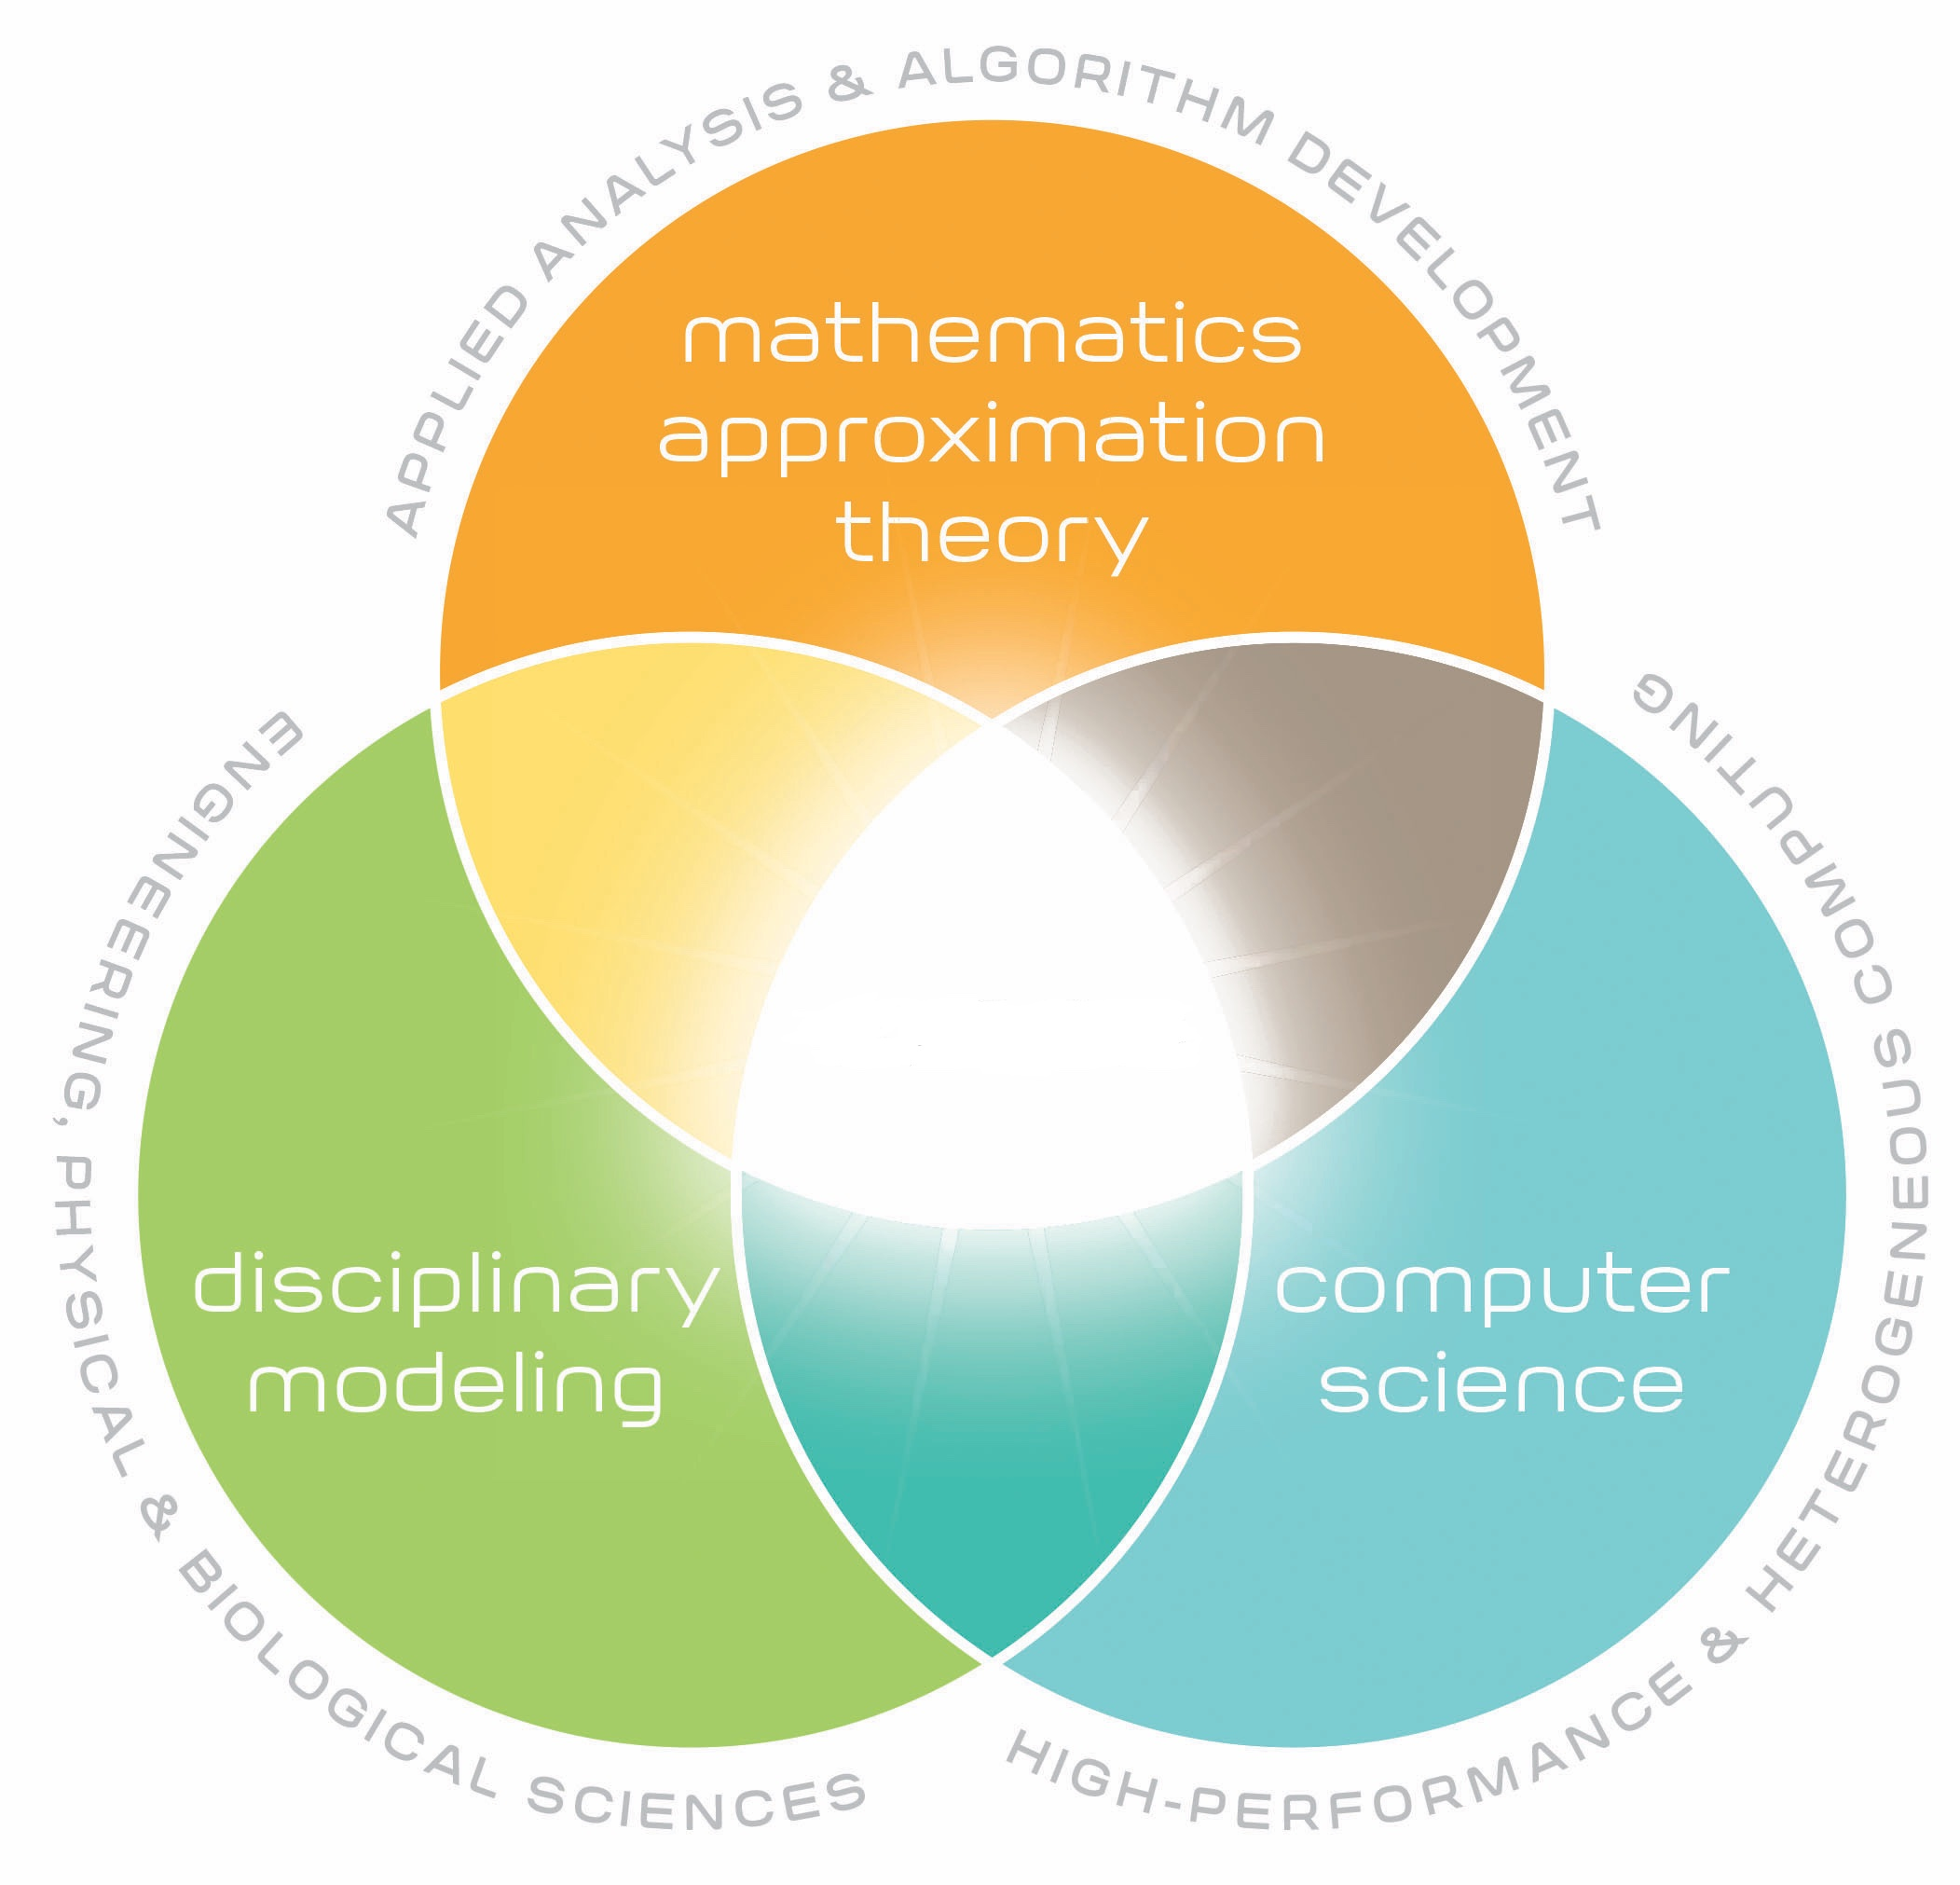
\includegraphics[width=.9\textwidth]{cse.jpg}
			\caption{\href{https://www.uio.no/english/studies/programmes/computational-science-master/why-choose/}{https://www.uio.no}}
		\end{figure}	
		\end{column}
		\begin{column}{.5\textwidth}
		Il s'agit d'une \textbf{sujet multidisciplinaire}, à l'intersection de\footnotemark :
		\begin{itemize}
			\item mathématiques appliquées (analyse numérique, discrétisation des EDP, optimisation);
			\item informatique et développement logiciel;
			\item modélisation physique.
		\end{itemize}
		
		\end{column}
	\end{columns}	
	\footcitetext{ulrich2018cse}
\end{frame}



\begin{frame}{Enjeux du poste}
	\centering
	\begin{tcolorbox}[hbox]
		\begin{tabular}{c|c}
			\textbf{Enseignant}	& \textbf{Chercheur}  \\
			\hline
			Formations	& Agenda de recherche \\
			Projets \& Stages	& Transversalité (ISAE)  \\
			Évolution programmes & Relations académiques\\
			& Partenariats Industrielles \\
			& Contrats de recherche \\
		\end{tabular}
	\end{tcolorbox}
\end{frame}


\section{Projet d'intégration}


\subsection{Missions enseignement}

\begin{frame}{Missions pour les poste E/C - Formation}

\begin{tcolorbox}
	Mission: \textcolor{blue}{\textbf{Intervention} dans les \textbf{formations} de l’ISAE SUPAERO}
\end{tcolorbox}

\only<1>{
\textbf{Compétences} : 
\begin{itemize}
	\item Méthodes numériques pour l'ingénieur (Formation ISAE, Stage CNES, Thèse, Post-Doc)
	\item Contrôle automatique et théorie des systèmes (Formation ISAE, Master recherche, Thèse, Conférences Internationales)
	\item Mécanique des solides et fluides (Licence, Thèse, Post-Doc) 
\end{itemize}
\vspace{.5cm}
\textbf{Expériences Enseignement} : 
\begin{itemize}
	\item 12h Mathématiques appliques (formation ISAE SUPAERO);
	\item 48h vacataire TP et BE en automatique (formation ISAE SUPAERO); 
	\item 40h vacataire TP et laboratoire expérimental en automatique (MAE);
\end{itemize}
}

\only<2>{
	\textbf{Formation ingénieur (FISE)}:
	\begin{itemize}
		\item 1A : Méthodes numériques EDO et EDP 1D (différences finies, éléments finis).
		\item 2A : Équations aux dérivées partielles - Théorie et simulations numériques.
		\item 3A : Domaine SXS 
		\begin{itemize}
			\item[--] Méthodes numériques pour la mécanique et la dynamique des fluides (éléments finis classiques et mixtes, volumes finis);
			\item[--] Calcul Haute performance (HPC);
		\end{itemize}
	\end{itemize}
	\vspace{.5cm}
	\textbf{Formation Master international MAE} :  EDP et calcul scientifique (en anglais).\\
	\vspace{.5cm}
	\textbf{Formation par Apprentissage (FISA)} : donner aux professionnels et apprentis les instruments nécessaires pour comprendre les logiciels des simulations.
}
\end{frame}


\begin{frame}{Missions pour le Poste E/C - Encadrement Projets}
	
	\begin{tcolorbox}
		Mission: \textcolor{blue}{\textbf{Encadrement} de projets d’\textbf{élèves}, de projets de recherche et de
		\textbf{stagiaires} au sein du DICS et \textbf{collaborations} avec les autres départements}
	\end{tcolorbox}

\textbf{Expériences} :
	\begin{itemize}
		\item \textbf{Organisation et encadrement du PIE} : "\textit{Simulation et contrôle des structures thermoélastiques pour applications spatiales}".
		\item \textbf{Supervision du PFE} de Vitor Borges Santos, en double diplôme ITA/UT Twente : "\textit{Model reduction for highly flexible thin structures}" (collaboration avec prof. Flavio Cardoso Ribeiro)
		\item \textbf{Supervision de la thèse} : "\textit{On the modeling and mechanical design of flexures (compliant mechanisms)}" (collaboration avec prof. Marijn Nijenhuis).
	\end{itemize}

\end{frame}


\begin{frame}{Missions pour le Poste E/C - Évolution Programmes}
	\begin{tcolorbox}
		Mission: \textcolor{blue}{\textbf{Contribuer à l’évolution et l’adaptation des programmes} en
		s’appuyant sur de nouvelles méthodes pédagogiques}
	\end{tcolorbox}

\textbf{Propositions} :

	
	\begin{itemize}
		\item \textbf{Création d'un gitlab commun de travail}, pour les \textbf{doctorants}, les \textbf{stagiaires} mais également pour le \textbf{BE} et \textbf{TP} des cours liés à la modélisation.
		\item \textbf{Organisation des conférences et séminaires} des experts dans le calcul scientifique pour l'ingénierie.
		\item \textbf{Intégration et continuation du module PFEM4PHS} : Modélisation et discrétisation symplectique des structures flexibles interconnectées.
		\item \textbf{Création du module électif} : Éléments de Géométrie différentielle pour la modélisation physique : du continu au discret.
	\end{itemize}
\end{frame}


\subsection{Missions recherche}

\begin{frame}{Missions pour le Poste E/C - Agenda de recherche}
	\begin{tcolorbox}
		Mission: \textcolor{blue}{Participation aux \textbf{activités de recherche} du DISC}
	\end{tcolorbox}

\only<1>{
\begin{itemize}
	\item \textbf{Modélisation et discrétisation structurées} des EDP (port-)Hamiltoniennes 
	\item \textbf{Applications} : mécanique, dynamique des fluides, électromagnétisme
\end{itemize}

\begin{columns}		
	\begin{column}{.3\textwidth}
		\includemedia[
		label=vidPlateRod,
		addresource=/home/andrea/Videos/CandidatureISAE/KirchhRod.mp4,
		activate=pageopen, 
		deactivate=onclick,
		width=5cm, height=5cm,
		flashvars={
			source=/home/andrea/Videos/CandidatureISAE/KirchhRod.mp4
			&%
			autoPlay=true&%
			loop=true%
		}
		]{}{VPlayer.swf}
		%\mediabutton[
		%mediacommand=vidPlateRod:playPause
		%]{\fbox{Play/Pause}}
		2D plaque interconnectée
	\end{column}
	\begin{column}{.3\textwidth}
		\includemedia[
		label=vidTG2D,
		addresource=/home/andrea/Videos/CandidatureISAE/vorticityTG2D.mp4,
		activate=pageopen, 
		deactivate=onclick,
		width=5cm, height=5cm,
		flashvars={
			source=/home/andrea/Videos/CandidatureISAE/vorticityTG2D.mp4&%
			autoPlay=true&%
			loop=true%
		}
		]{}{VPlayer.swf}
		%\mediabutton[
		%mediacommand=vidTG2D:playPause
		%]{\fbox{Play/Pause}}
		2D Hydrodynamique
	\end{column}
	\begin{column}{.3\textwidth}
		\includemedia[
		label=vidMaxwell3D,
		addresource=/home/andrea/Videos/CandidatureISAE/MaxwellE13D.mp4,
		activate=pageopen, 
		deactivate=onclick,
		width=5cm, height=5cm,
		flashvars={
			source=/home/andrea/Videos/CandidatureISAE/MaxwellE13D.mp4
			&%
			autoPlay=true&%
			loop=true%
		}
		]{}{VPlayer.swf}
		%\mediabutton[
		%mediacommand=vidMaxwell3D:playPause,
		%]{\fbox{Play/Pause}}
		3D Maxwell
	\end{column}
\end{columns}	
%\mediabutton[
%mediacommand=vidPlateRod:playPause,
%overface=\color{blue}{\fbox{\strut Play/Pause}},
%downface=\color{red}{\fbox{\strut Play/Pause}}
%]{\fbox{\strut Play/Pause}}

%\mediabutton[
%mediacommand=vidPlateRod:setSource [(KirchhRod.mp4)]
%]{\fbox{\strut KirchhRod.mp4}}
}

\only<2>{
\begin{block}{Nouvelles pistes}
	\begin{itemize}
		\item \textbf{Analyse} des schémas numériques.
		\item Lien entre \textbf{géométrie et discrétisation} : \textit{les éléments finis en calcul extérieur}.
		\item Stratégies pour le \textbf{gain en performance} : maillage adaptatif, solveurs et preconditionneurs, parallélisation du code et calcul haute performance. 
		\item Lien avec l'\textbf{intelligence artificielle et compression de données}.
	\end{itemize}
	
	
\end{block}


\begin{block}{Développement logiciel}
	\begin{itemize}
		\item Développement d'un code de calcul pour la multiphysique (SCRIMP).
		\item Intégrations des algorithmes de réductions de modèles et optimisation.
	\end{itemize}	
	
\end{block}
}
\end{frame}


\begin{frame}{Missions pour le Poste E/C - Transversalité}
	\begin{tcolorbox}
		Mission: \textcolor{blue}{Développer la \textbf{recherche} d'une manière \textbf{transversale} au sein du DISC et des autres départements}
	\end{tcolorbox}

	\textbf{Transversalité DISC} : 
	\begin{itemize}
		\item L'\textbf{intelligence artificielle} offre des outils essentiels pour la \textbf{compression de données} issus des schémas de discrétisation.
		\item \textbf{Ouverture} vers le \textbf{stochastique} : modélisation d'\textbf{incertitude} au sein des \textbf{modèles physiques}.
	\end{itemize}
	
	
	\textbf{Collaborations} avec d'autres départements :
	\begin{itemize}
		\item \textbf{DMSM} : mécanique structurelle et optimisation topologique. 
		\item \textbf{DCAS} : réduction des modèles et le contrôle automatique.
		\item \textbf{DAEP} : dynamique des fluides computationnelle.
	\end{itemize}
	
\end{frame}



\begin{frame}{Missions pour le Poste E/C - Relations Académique}
	\begin{tcolorbox}
	Mission: \textcolor{blue}{\textbf{Ouverture de collaborations} avec partenaires \textbf{académiques}}
	\end{tcolorbox}
	
	
	\textbf{Collaborations Existantes et Historiques} 
	\begin{figure}[t]
		\begin{subfigure}{0.5\textwidth}
			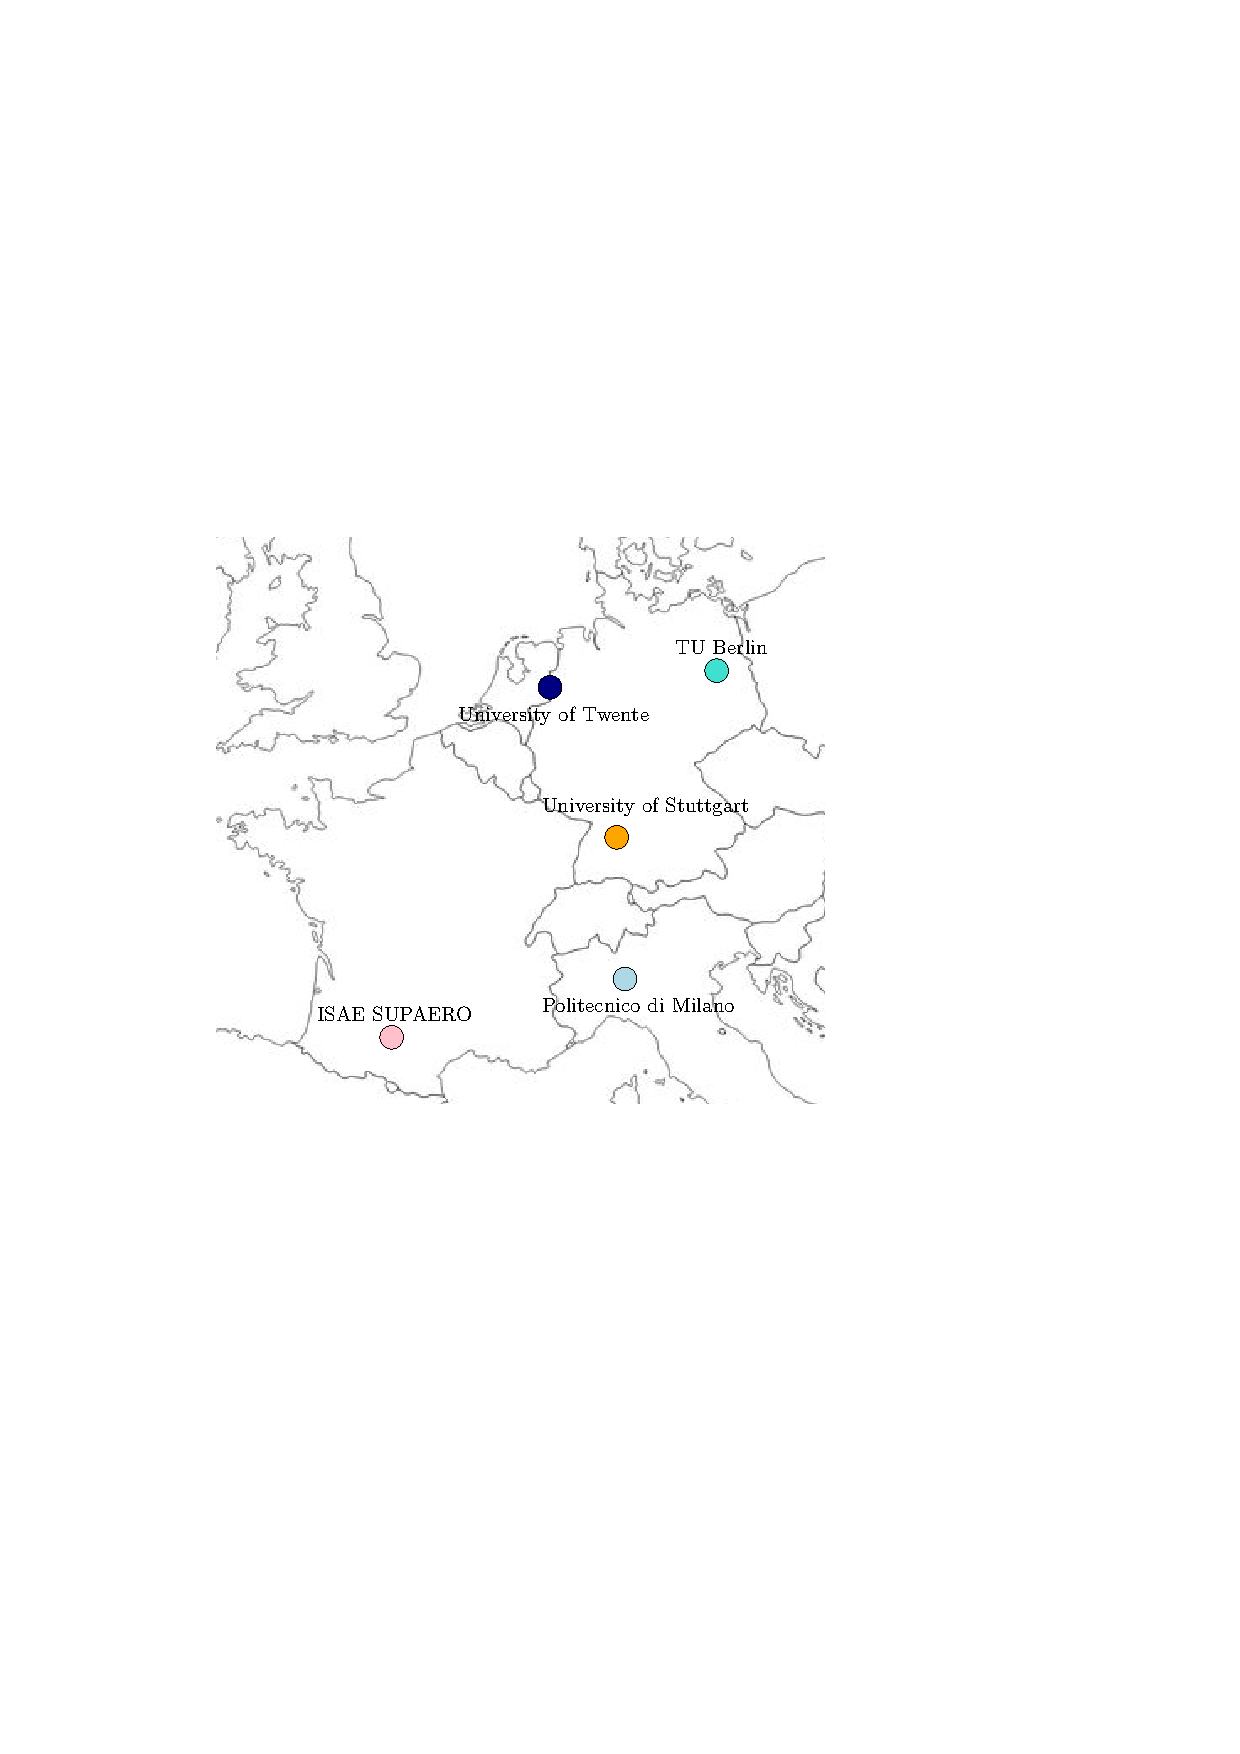
\includegraphics[height=.6\textheight]{mappe_reseau_europe.pdf}%
		\end{subfigure}\hfill
		\begin{subfigure}{0.4\textwidth}
			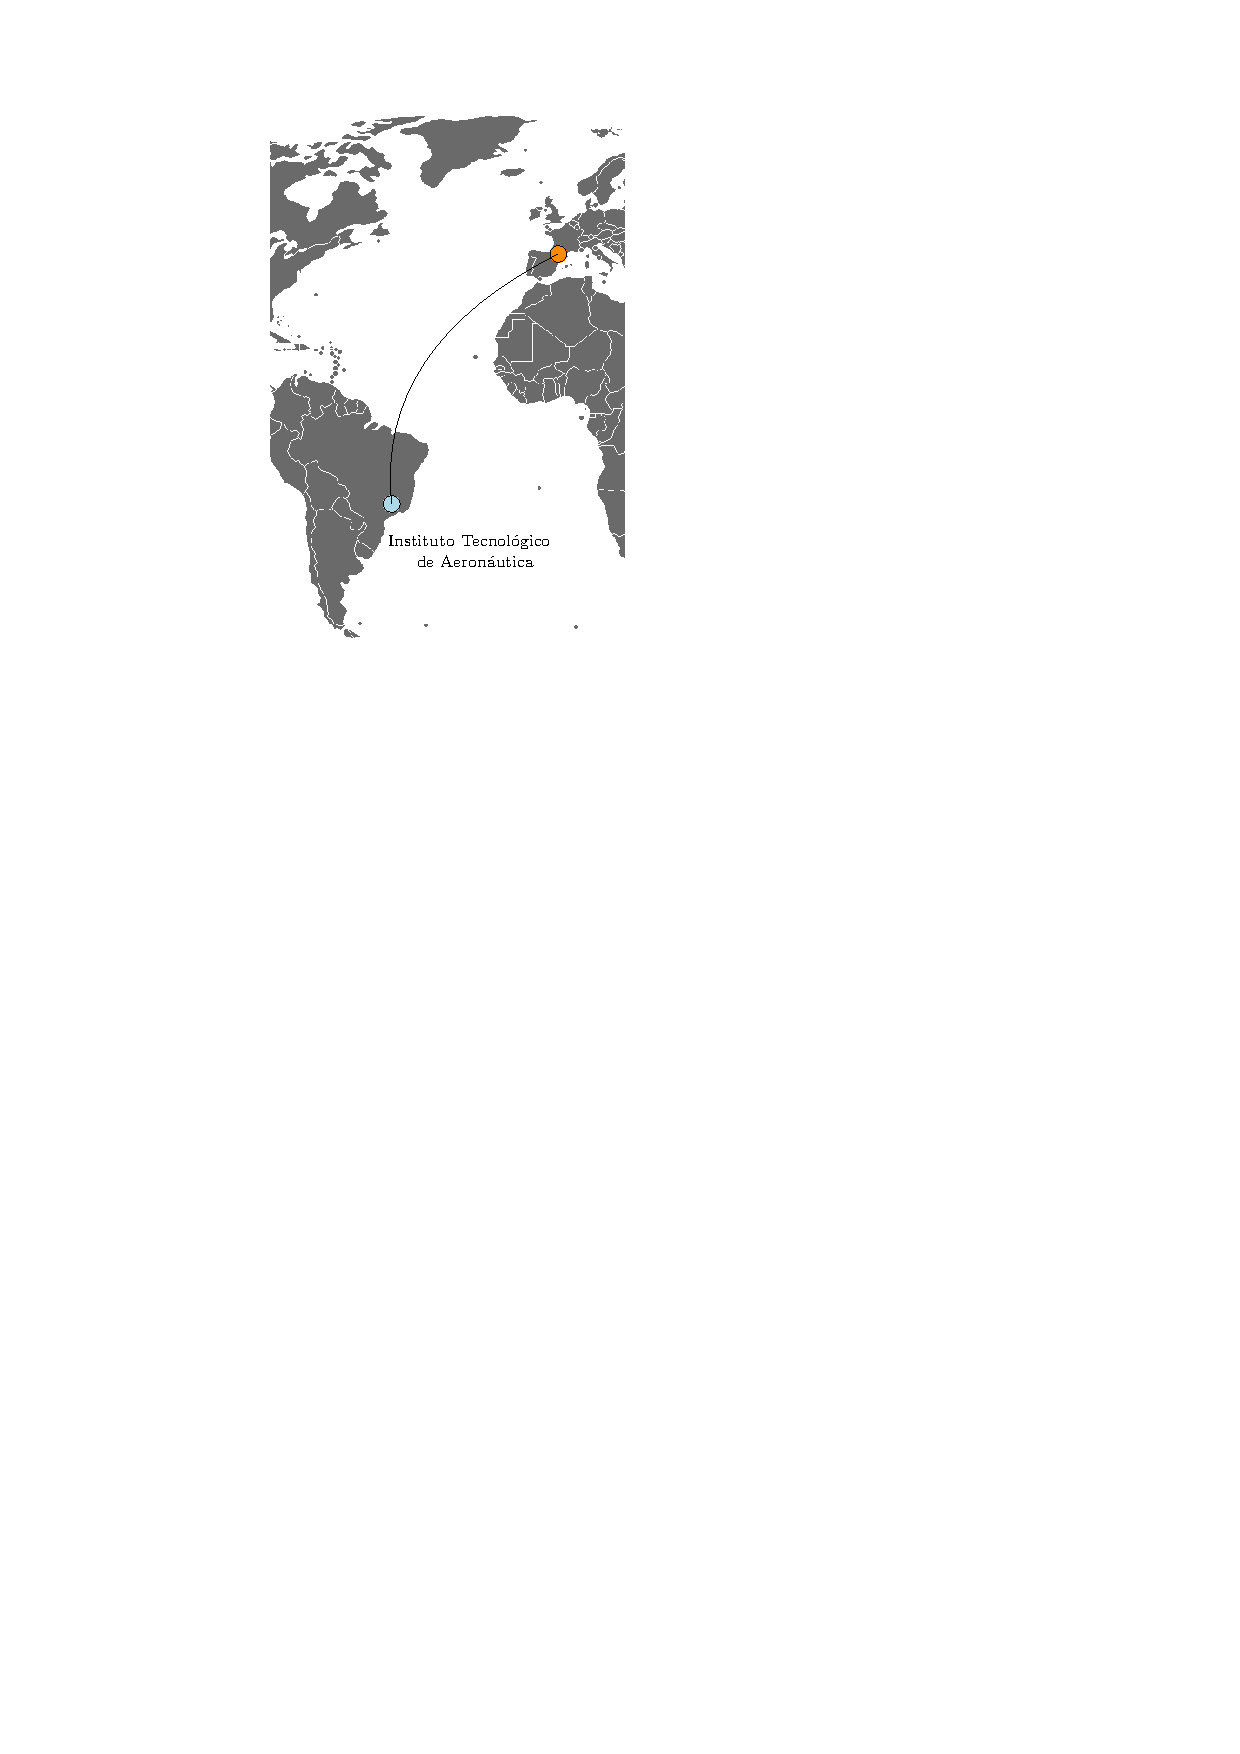
\includegraphics[height=.65\textheight]{mappe_reseau_world.pdf} 
		\end{subfigure}
	\end{figure}
\end{frame}


\begin{frame}{Missions pour le Poste E/C - Partenariats industrielles}	

	\begin{tcolorbox}
		Mission: \textcolor{blue}{\textbf{Développement} des partenariats industriels}
	\end{tcolorbox}

	\begin{columns}
		\begin{column}{.5\textwidth}
			\textbf{Manifestation d'intérêt} : 
			\begin{itemize}
				\item \textbf{CEA} : simulation multiphysique.
				\item \textbf{CERFACS} : CFD et assimilation des données. 
				\item \textbf{AIRBUS} : aéroélasticité et mécanique.
			\end{itemize}
		\textbf{Partenariats} industriels \textbf{potentielles} : 
		\begin{itemize}
			\item  \textbf{THALES} : électromagnétisme, thermoélasticité.
		\end{itemize}
		\end{column}
		\begin{column}{.43\textwidth}
			\begin{figure}
				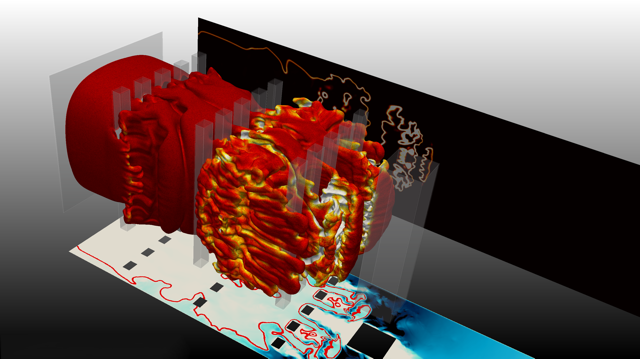
\includegraphics[width=1\textwidth]{image_CERFACS.png}
				\caption{\href{https://cerfacs.fr/logiciels-de-simulation-pour-la-mecanique-des-fluides/}{https://cerfacs.fr}}
			\end{figure}	
		\end{column}
	\end{columns}
	
\end{frame}




\begin{frame}{Missions pour le Poste E/C - Contrats de recherche}	
\begin{tcolorbox}
Mission : \textcolor{blue}{Proposition et \textbf{développement de contrats de recherche}}
\end{tcolorbox}
\textbf{Projets} : 
\begin{itemize}
	\item Agence nationale de la recherche (ANR): Domaine "Sciences du numérique".
	\item Financement ERC (European Research Council).
\end{itemize}

\textbf{Thèses} : sources de financement ou co-financement
\begin{itemize}
\item Horizon 2024 : Marie Sklodowska-Curie Actions (MSCA) PhD Funding;
\item Appel à projets de Recherche (APR);
\item Région "Allocations doctorales"
\end{itemize}

\end{frame}

\begin{frame}{}
	\centering
	\Large Merci de votre attention
\end{frame}

\appendix

\begin{frame}{}
	\centering
	\Huge{Annexe}
\end{frame}

\section{Formation et Expériences}

\begin{frame}{Parcours académique}
\begin{itemize}
	\item (2011-2014) \textbf{Licence en génie mécanique}, Politecnico di Milano;
	\item (2014-2017) \textbf{Master en génie spatial}, Politecnico dI Milano;
	\item (2014-2017) \textbf{Diplôme d’Ingénieur Supaéro}, Programme de
	Double Diplôme, ISAE SUPAERO/Politecnico di Milano;
	\item (2016-2017) \textbf{Master recherche en automatique et traitement d’images
	} ISAE-SUPAERO/SUPELEC (Université Paris Saclay);
	\item (2017-2020) \textbf{Thèse} : "\textit{Une formulation port-Hamiltonienne des structures flexibles. Modélisation et discrétisation symplectique par éléments finis}", ISAE-SUPAERO.
\end{itemize}
\end{frame}

\begin{frame}{Expériences}
\begin{itemize}
\item (2014 : 4 mois) \textbf{Projet Fin Études (Licence)} : \textit{Dynamique d’un manipulateur pour machines de forgeage}, Danieli SPA, Buttrio (Italie);
\item (2017 : 6 mois) \textbf{Projet Fin Études (Master)} : \textit{Analyse de la dynamique des débris spatiaux soumis à la pression de radiation solaire}, CNES, Toulouse (France)
\item (2019 : 4 mois) \textbf{Chercheur invité} : \textit{Collaboration avec prof. Flavio Cardoso-Riberio}, Instituto Tecnológico de Aeronáutica (Brésil);
\item (2020-2022) : \textbf{Chercheur post-doctoral} : \textit{Méthodes numériques pour problèmes couplés fluide-structure}, ERC avancé, PI Stefano Stramigioli, Enschede (Pays-Bas);
\item (Juillet 2021 : 1 semaine) \textbf{École d'été} : \textit{Intelligence artificielle et apprentissage par renforcement}, Institut Cifar, Toronto (Canada);
\item (Avril 2022 : 1 semaine) \textbf{Invitation au CIRM} (centre international de rencontre mathématiques) : \textit{Modélisation structurée, intégration géométrique et commande de systèmes multiphysiques contraints}, Marseille (France).
\end{itemize}
  
\end{frame}

\section{Production scientifiques}

\begin{frame}{Articles de revue (mathématiques appliquées)}
\begin{enumerate}
	\item \cite{brugnoli2022df}
	\item \cite{brugnoli2021num}
	\item \cite{brugnoli2019ammmin}
	\item \cite{brugnoli2019ammkir}
\end{enumerate}


\end{frame}


\begin{frame}{Congres internationales (mathématiques appliquées)}
\footnotesize	
\begin{enumerate}
	\item \cite{brugnoli2021vk}
	\item \cite{rashad2021ext}
	\item \cite{cherifi2021data}
	\item \cite{brugnoli2021siamcse}
	\item \cite{brugnoli2020mtns}
	\item \cite{brugnoli2019cpde}
\end{enumerate}

\end{frame}

\begin{frame}{Articles de revue et Congres internationales (mécanique et automatique)}
	\textbf{Articles de revue} : 
	\begin{enumerate}
		\item \cite{brugnoli2021ther}
		\item \cite{brugnoli2020msd}
	\end{enumerate}
	\textbf{Congres internationales} :
	\begin{enumerate}
		\item \cite{brugnoli2019cdc}
		\item \cite{cardoso2019cdc}
	\end{enumerate}
\end{frame}

\section{Résume activités enseignement et scientifiques}

\begin{frame}{Résumé activité d'enseignement}
	\begin{table}
		\centering
		\begin{tabular}{p{\dimexpr.15\linewidth-2\tabcolsep}p{\dimexpr.15\linewidth-2\tabcolsep}p{\dimexpr.15\linewidth-2\tabcolsep}p{\dimexpr.4\linewidth-2\tabcolsep}p{\dimexpr.15\linewidth-2\tabcolsep}}
			\hline
			Année & Niveau & Nature  & Discipline & Durée  \\
			\hline
			\multirow{2}{*}{2019-2020} & L1 & TD &  Résolution numérique des EDP & 6h \\
			& L1 & TD &  Optimisation & 6h \\
			\hline
			\multirow{3}{*}{2018-2019} & L2  & TP-TD  & Automatique & 20h \\
			& L2  & TD     & Contrôle des structures flexibles & 8h \\
			& L2  & TP-TD  & Automatic control & 20h \\
			\hline
			\multirow{2}{*}{2017-2018} & L2  & TP-TD  & Automatique & 20h \\
			& L2  & TP-TD  & Automatic control & 20h \\				   
			\hline
		\end{tabular}


	\end{table}
\end{frame}

\begin{frame}{Résumé des activité scientifiques.}
	\small
	\begin{table}
		\centering
		\begin{tabular}{p{\dimexpr.15\linewidth-2\tabcolsep}p{\dimexpr.2\linewidth-2\tabcolsep}p{\dimexpr.65\linewidth-2\tabcolsep}}
			\hline
			Année & Lieu & Description  \\
			\hline
			2022 (en cours) & University of Twente (Enschede) & Supervision du projet fin étude de Vitor Borges Santos dans le cadre du double diplôme ITA/UT Twente (collaboration avec prof. Flavio Cardoso Ribeiro). \\
			2022 (en cours) & University of Twente (Enschede) & Supervision de la thèse "On the modeling and mechanical design of flexures (compliant mechanisms)" (collaboration avec prof. Marijn Nijenhuis). \\
			\hline
			2021  & Technical University of Berlin (Berlin) & Organisation de la session invitée: "Theoretical and numerical advancements in Hamiltonian formulations of continuum mechanics" pour la conférence "Lagrangian and Hamiltonian method in non linear control 2021". \\
			\hline
			2020 & --- & Critiques (Peer reviews) des journaux \textit{Journal of Elasticity} et \textit{Mathematical and Computer Modelling of Dynamical Systems} et conférences LHMNC, MATHMOD, MTNS. \\
			\hline
			2019-2020 & ISAE-SUPAERO (Toulouse) & Organisation et encadrement du Projet Ingénierie et Entreprise intitulé "Simulation et contrôle des structures thermoélastiques pour
			applications spatiales". \\
			\hline
		\end{tabular}

		\label{tab:activites}
	\end{table}
\end{frame}


\section{Détails transversalité ISAE}

\begin{frame}{Transversalité (DISC)}
	L'\textbf{intelligence artificielle} offre des outils essentiels pour la compression de données issus des schémas de discrétisation.
	
	\begin{figure}[t]
		\begin{subfigure}[t]{0.48\textwidth}
			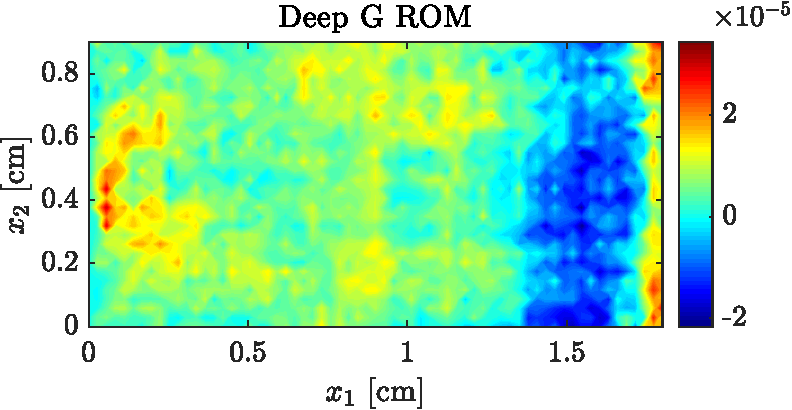
\includegraphics[width=\columnwidth]{DGROM_T_param1.pdf} 
			\caption*{Modèle réduit avec réseaux des neurones.}
		\end{subfigure}\hfill
		\begin{subfigure}[t]{0.48\textwidth}
			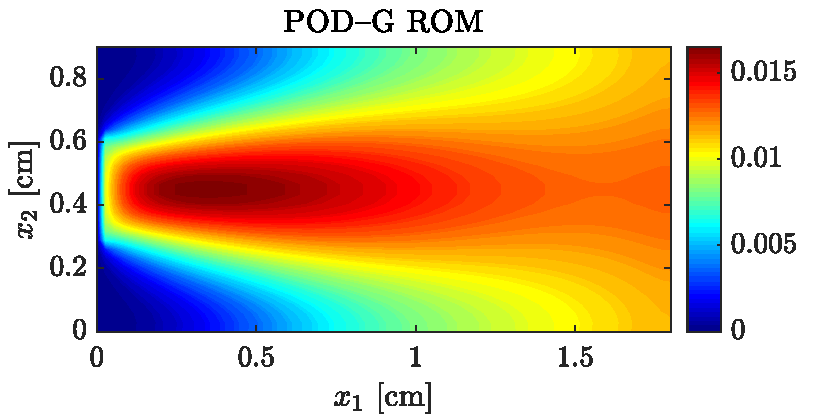
\includegraphics[width=\columnwidth]{GROM_T_param1.pdf}%
			\caption*{Modèle réduit avec la méthode linéaire POD.}
		\end{subfigure}
		\caption*{Erreur des modèles réduits sur le champ de température pour un problème de convection-diffusion-réaction (Reproduit avec permission de \cite{lee2020}).}%
	\end{figure}
\end{frame}


\begin{frame}{Transversalité (ISAE)}
	\textbf{Exemples de cas d'application} où le calcul scientifique est fondamental :
	\begin{figure}[t]
		\begin{subfigure}{0.45\textwidth}
			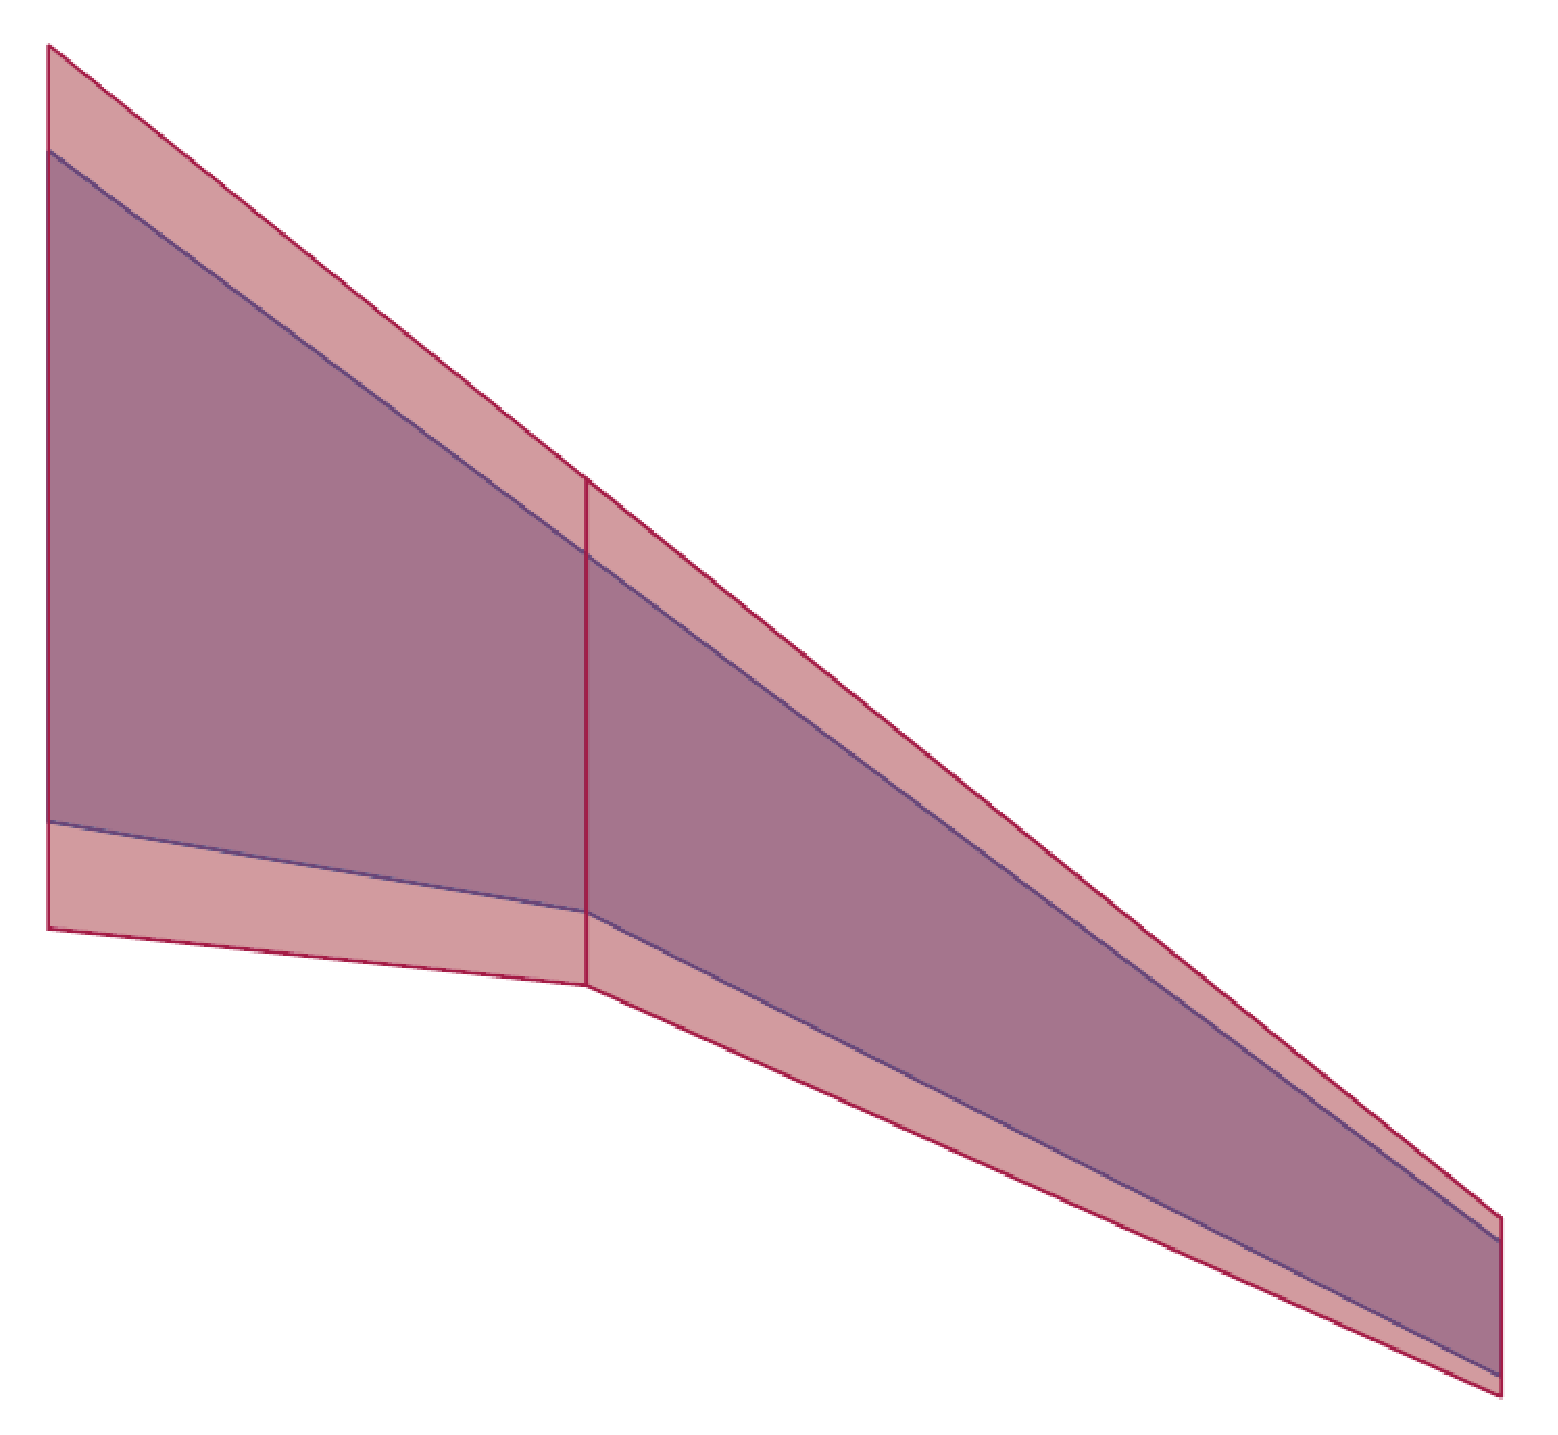
\includegraphics[height=.45\textheight]{MDO_wing.pdf}%
			\caption*{\textbf{Optimisation multidisciplinaire d'une aile} (\cite{masColomer2021mdo}). }
		\end{subfigure}\hfill
		\begin{subfigure}{0.5\textwidth}
			\includegraphics[height=.45\textheight]{Codesign_satellite.pdf} 
			\caption*{\textbf{Co-design contrôle/structure pour un satellite} (\cite{finozzi2022sub}).}
		\end{subfigure}
	\end{figure}
	
\end{frame}

\section{Détails projets de thèses et collaborations industrielles}

\begin{frame}{Méthodes numériques pour problèmes couplés multiphysiques}
	Le \textbf{CEA} a manifesté son intérêt pour l'utilisation du paradigme port-Hamiltonien pour la discrétisation structuré des systèmes couplés.
	
	\begin{block}{Projet de thèse chiffre ISAE-CEA}
		\textit{Discrétisation géométrique par éléments finis pour la Magnétohydrodynamique.}
	\end{block}
	
	\begin{tcolorbox}
		La plupart des méthodes utilisées en MHD computationnel reprennent des techniques bien établies employées en dynamique des fluides. Un problématique fondamental est la préservation de la nature solénoïdal du champ magnétique\footnote{\url{https://en.wikipedia.org/wiki/Computational_magnetohydrodynamics}}. Une discrétisation géométrique basée sur les éléments offre une piste une recherche intéressante pour la conception des schémas plus performants \footcite{hiptmair2018div}.
	\end{tcolorbox}	
	
\end{frame}

\begin{frame}{Réduction de modèle structurée par réseaux des neurones}
	Le \textbf{CERFACS} (équipe Hélios) s'intéressent à l'intégration d'outils issus de l'Intelligence Artificielle pour accélérer le code des calculs pour la dynamique des fluides.
	
	\begin{block}{Projet de thèse chiffre ISAE-CERFACS}
		\textit{Réduction de modèles pour la dynamique des fluides au delà des approches linéaires}
	\end{block}
	\begin{tcolorbox}
		La grande majorité de ces méthodes suppose que l’on puisse obtenir un système réduit à travers une méthode essentiellement linéaire, i.e. la Décomposition Orthogonale en Valeurs Propres (POD). Cette hypothèse n’est pas valable pour tout système exhibant un comportement non-linéaire et
		conduit à surestimer la dimension du système réduit. Dans le domaine de l’Intelligence Artificielle (IA), de nouvelles méthodes permettent d’obtenir des modèles réduits plus performants\footcite{lee2020}.
	\end{tcolorbox}
	
\end{frame}

\section{Détails Activités recherches récentes}

\begin{frame}{Activités recherche post Doc}
Discrétisation géométrique des systèmes port-Hamiltoniens. \\
\textbf{Équation d'onde }

\only<1>{
	
	\begin{columns}		
		\begin{column}{.45\textwidth}
			\includemedia[
			addresource=/home/andrea/Videos/CandidatureISAE/Wavep33D.mp4,
			activate=pageopen, 
			deactivate=onclick,
			width=7cm, height=6cm,
			flashvars={
				source=/home/andrea/Videos/CandidatureISAE/Wavep33D.mp4
				&%
				autoPlay=true&%
				loop=true%
			}
			]{}{VPlayer.swf}
			Pression 3 forme
		\end{column}
		\begin{column}{.45\textwidth}
			\includemedia[
			addresource=/home/andrea/Videos/CandidatureISAE/Wavep03D.mp4,
			activate=pageopen, 
			deactivate=onclick,
			width=7cm, height=6cm,
			flashvars={
				source=/home/andrea/Videos/CandidatureISAE/Wavep03D.mp4&%
				autoPlay=true&%
				loop=true%
			}
			]{}{VPlayer.swf}
			Pression 0 forme
		\end{column}
	\end{columns}	
}

\only<2>{
	
	\begin{columns}		
		\begin{column}{.45\textwidth}
			\includemedia[
			addresource=/home/andrea/Videos/CandidatureISAE/Waveu23D.mp4,
			activate=pageopen, 
			deactivate=onclick,
			width=7cm, height=6cm,
			flashvars={
				source=/home/andrea/Videos/CandidatureISAE/Waveu23D.mp4
				&%
				autoPlay=true&%
				loop=true%
			}
			]{}{VPlayer.swf}
			Vitesse 2 forme
		\end{column}
		\begin{column}{.45\textwidth}
			\includemedia[
			addresource=/home/andrea/Videos/CandidatureISAE/Waveu13D.mp4,
			activate=pageopen, 
			deactivate=onclick,
			width=7cm, height=6cm,
			flashvars={
				source=/home/andrea/Videos/CandidatureISAE/Waveu13D.mp4&%
				autoPlay=true&%
				loop=true%
			}
			]{}{VPlayer.swf}
			Vitesse 1 forme
		\end{column}
		
	\end{columns}	
}
	
\only<3>{	
\begin{figure}
\centering
\subfloat[][Erreur $L^2$ pour $p^3_h$]{%
	\label{fig:err_p3}%
	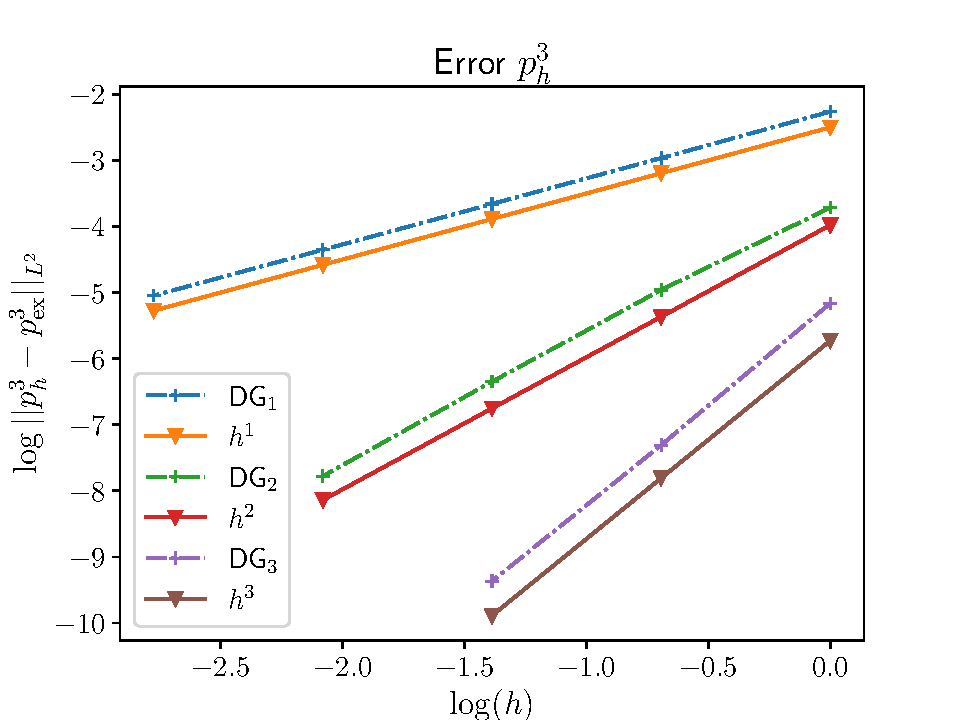
\includegraphics[width=0.48\columnwidth]{p_3_3D_DN.pdf}}%
\hspace{8pt}%
\subfloat[][Erreur $L^2$ pour $p^0_h$]{%
	\label{fig:err_p0}%
	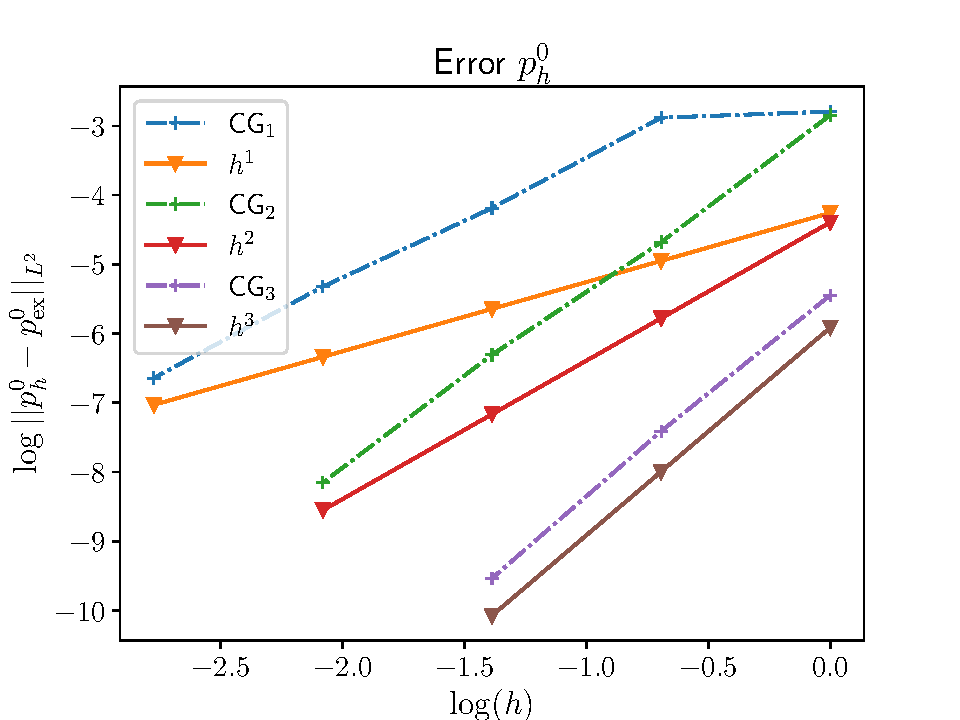
\includegraphics[width=0.48\columnwidth]{p_0_3D_DN.pdf}}%
\caption*{Pente de convergence pour la rapresentation duale de la pression}%
\end{figure}
}
\only<4>{	
\begin{figure}
	\centering
	\subfloat[][Erreur $L^2$ pour $u^1_h$]{%
		\label{fig:err_u1}%
		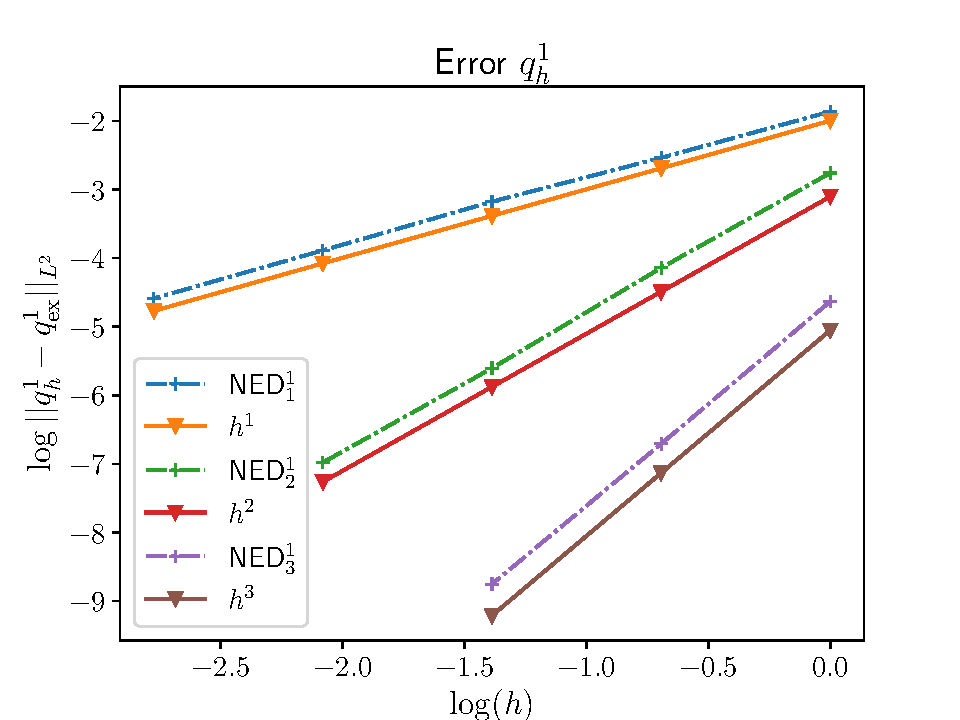
\includegraphics[width=0.48\columnwidth]{q_1_3D_DN.pdf}}
	\hspace{8pt}%
	\subfloat[][Erreur $L^2$ pour $u^2_h$]{%
		\label{fig:err_u2}%
		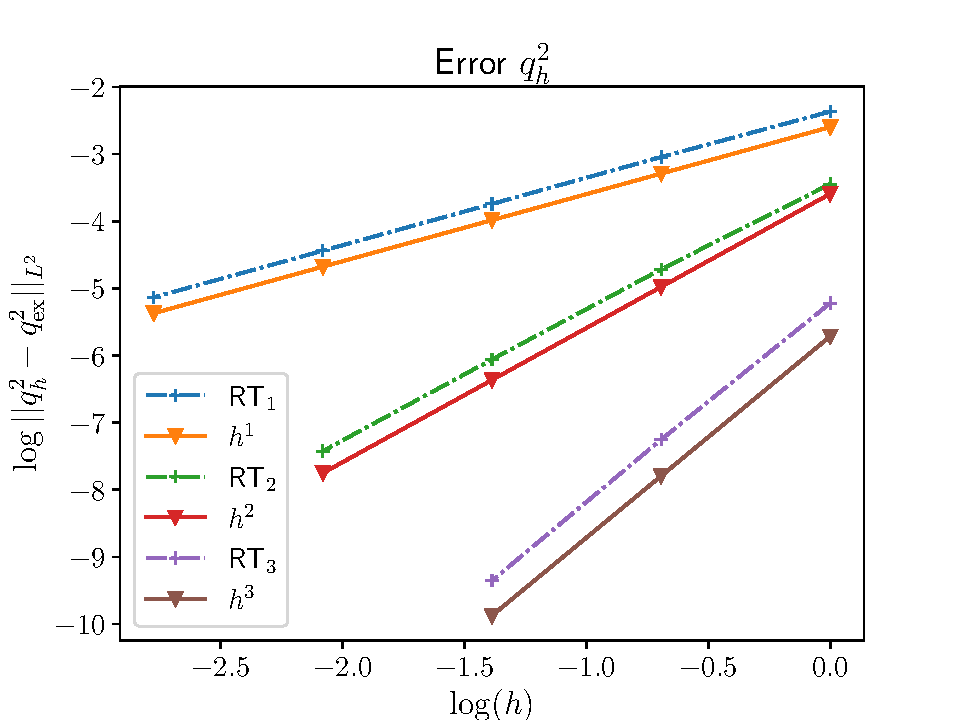
\includegraphics[width=0.48\columnwidth]{q_2_3D_DN.pdf}}
	\caption*{Pente de convergence pour la rapresentation duale de la vitesse}%
\end{figure}
}
\only<5>{
\begin{figure}
	\centering
	\subfloat[][Norme $L^2$ de la difference $p^3_h - p^0_h$]{%
		\label{fig:diff_p30}%
		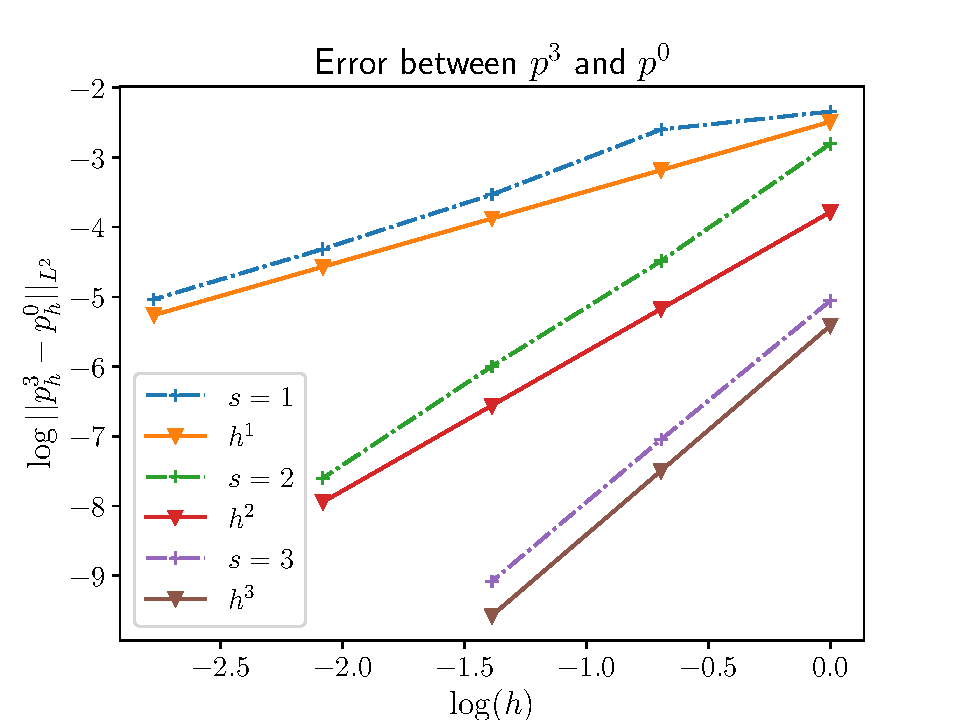
\includegraphics[width=0.48\columnwidth]{p_30_3D_DN.pdf}}%
	\hspace{8pt}%
	\subfloat[][Norme $L^2$ de la difference $q^1_h - q^2_h$]{%
		\label{fig:diff_q12}%
		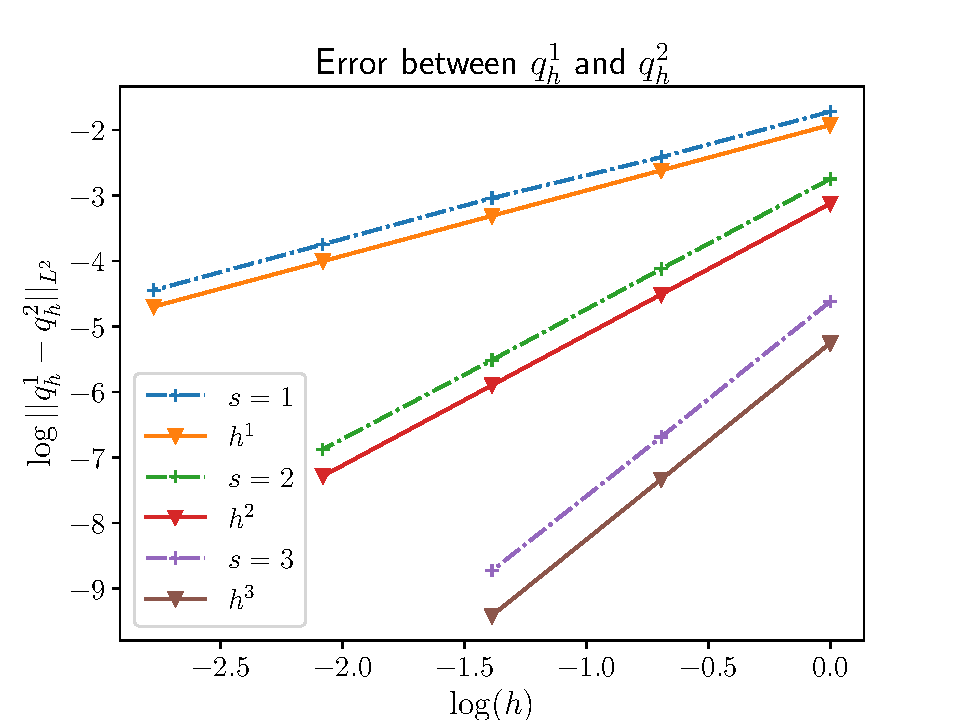
\includegraphics[width=0.48\columnwidth]{q_12_3D_DN.pdf}}%
	\caption*{Différence $L^2$ pour la représentation duale des variables.}%
\end{figure}
}



\end{frame}

\begin{frame}{Activités recherche post Doc}
	Discrétisation géométrique des systèmes port-Hamiltoniens. \\
	\textbf{Équation de Maxwell}
	
	\only<1>{
		
		\begin{columns}		
			\begin{column}{.45\textwidth}
				\includemedia[
				addresource=/home/andrea/Videos/CandidatureISAE/MaxwellE23D.mp4,
				activate=pageopen, 
				deactivate=onclick,
				width=7cm, height=6cm,
				flashvars={
					source=/home/andrea/Videos/CandidatureISAE/MaxwellE23D.mp4
					&%
					autoPlay=true&%
					loop=true%
				}
				]{}{VPlayer.swf}
				Champ électrique 2 forme
			\end{column}
			\begin{column}{.45\textwidth}
				\includemedia[
				addresource=/home/andrea/Videos/CandidatureISAE/MaxwellE13D.mp4,
				activate=pageopen, 
				deactivate=onclick,
				width=7cm, height=6cm,
				flashvars={
					source=/home/andrea/Videos/CandidatureISAE/MaxwellE13D.mp4&%
					autoPlay=true&%
					loop=true%
				}
				]{}{VPlayer.swf}
				Champ électrique 1 forme
			\end{column}
			
		\end{columns}	
	}
	
	\only<2>{	
		\begin{figure}
			\centering
			\subfloat[][Erreur $L^2$ pour $E^2_h$]{%
				\label{fig:err_E2}%
				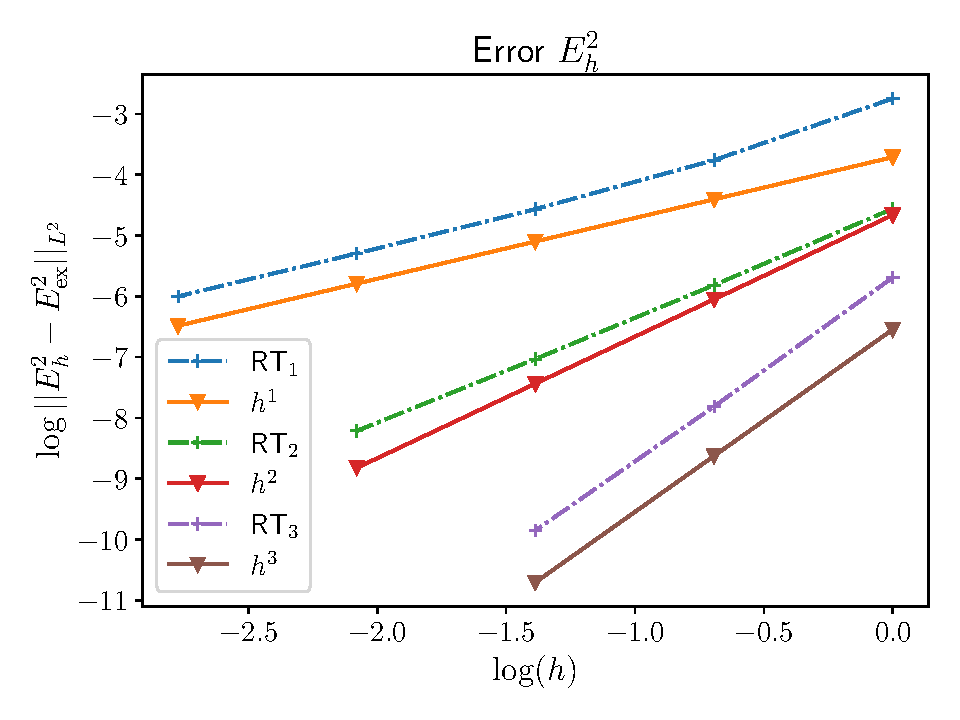
\includegraphics[width=0.48\columnwidth]{E_2_3D_EH.pdf}}%
			\hspace{8pt}%
			\subfloat[][Erreur $L^2$ pour $E^1_h$]{%
				\label{fig:err_E1}%
				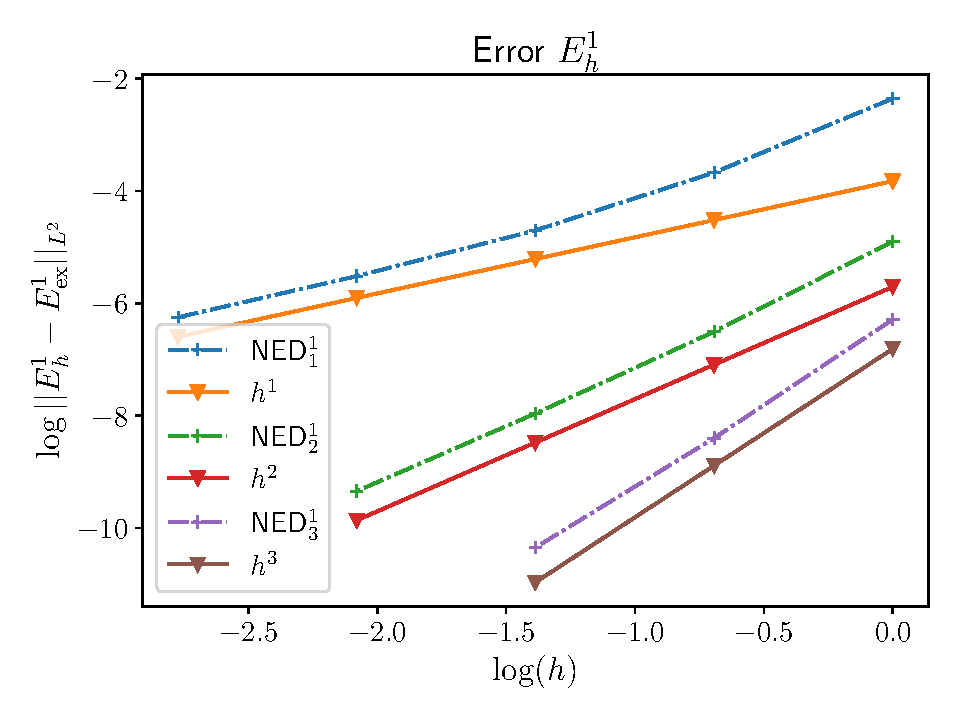
\includegraphics[width=0.48\columnwidth]{E_1_3D_EH.pdf}}%
			\caption{Pente de convergence pour la représentation duale du champ Électrique}%
		\end{figure}
	}
	\only<3>{	
		\begin{figure}
			\subfloat[][Erreur $L^2$ pour $H^2_h$]{%
				\label{fig:err_H2}%
				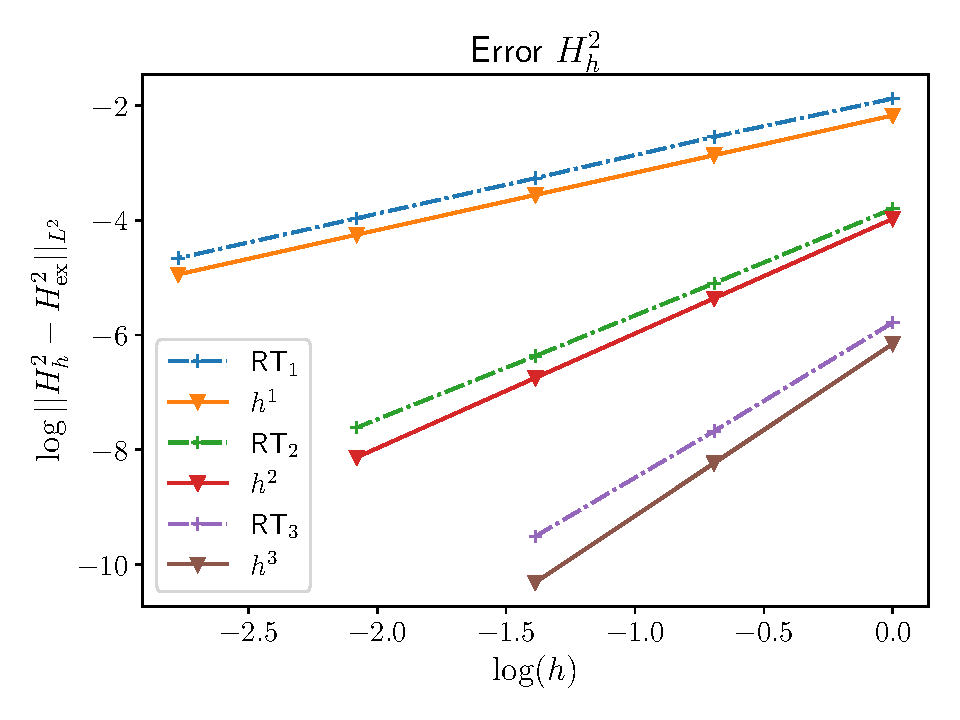
\includegraphics[width=0.48\columnwidth]{H_2_3D_EH.pdf}}
			\hspace{8pt}%
			\subfloat[][Erreur $L^2$ error for $H^1_h$]{%
				\label{fig:err_H1}%
				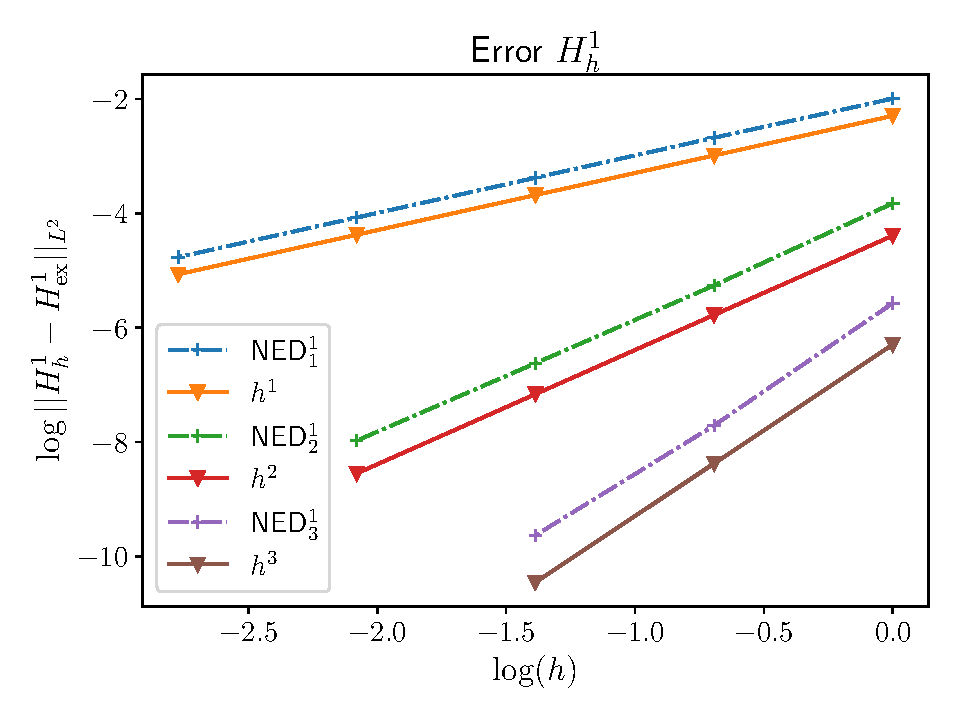
\includegraphics[width=0.48\columnwidth]{H_1_3D_EH.pdf}}
			\caption{Pente de convergence pour la représentation duale du champ Magnétisant}%
		\end{figure}
	}
	\only<4>{
		\begin{figure}
			\centering
			\subfloat[][$L^2$ norm of the difference $E^1_h - E^2_h$]{%
				\label{fig:diff_E21}%
				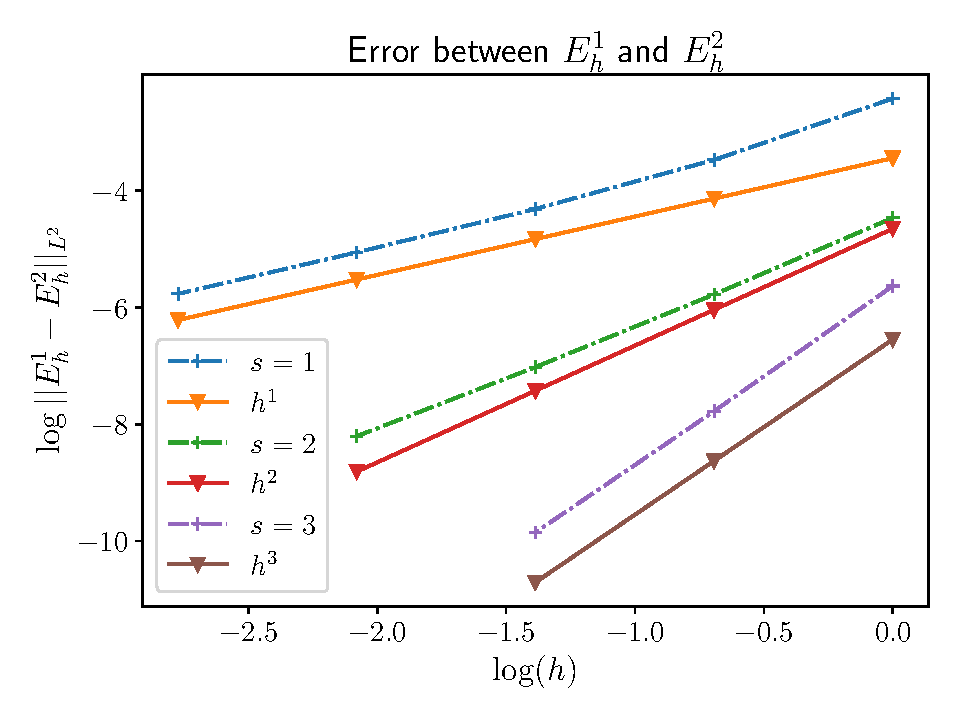
\includegraphics[width=0.48\columnwidth]{E_21_3D_EH.pdf}}%
			\hspace{8pt}%
			\subfloat[][$L^2$ norm of the difference $H^1_h - H^2_h$]{%
				\label{fig:diff_H21}%
				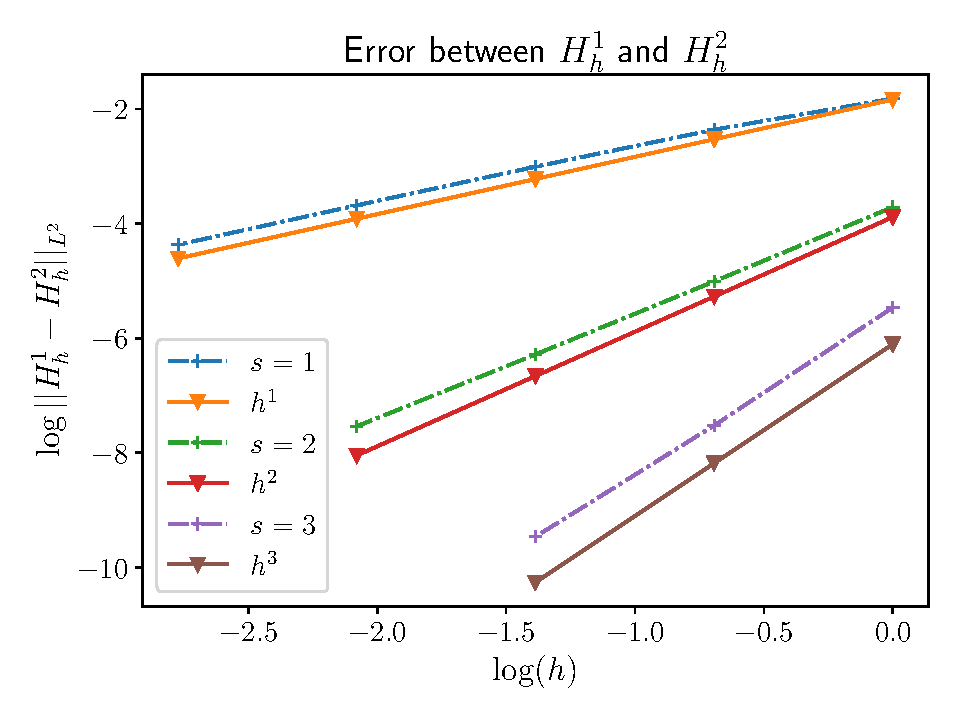
\includegraphics[width=0.48\columnwidth]{H_21_3D_EH.pdf}}%
			\caption*{Différence $L^2$ pour la représentation duale des variables.}%
		\end{figure}
	}

	
\end{frame}





\end{document}